\begin{frame}

	\frametitle{From Voxel to Mesh Geometry}
	\begin{minipage}{0.85\textwidth}
		\begin{itemize}
		\item Extract isosurface from voxel information
		\item Algorithms: Marching Cubes, Dual Contouring, Extended Models
		\item Implementations in VTK library
		\end{itemize}

		\begin{figure}
		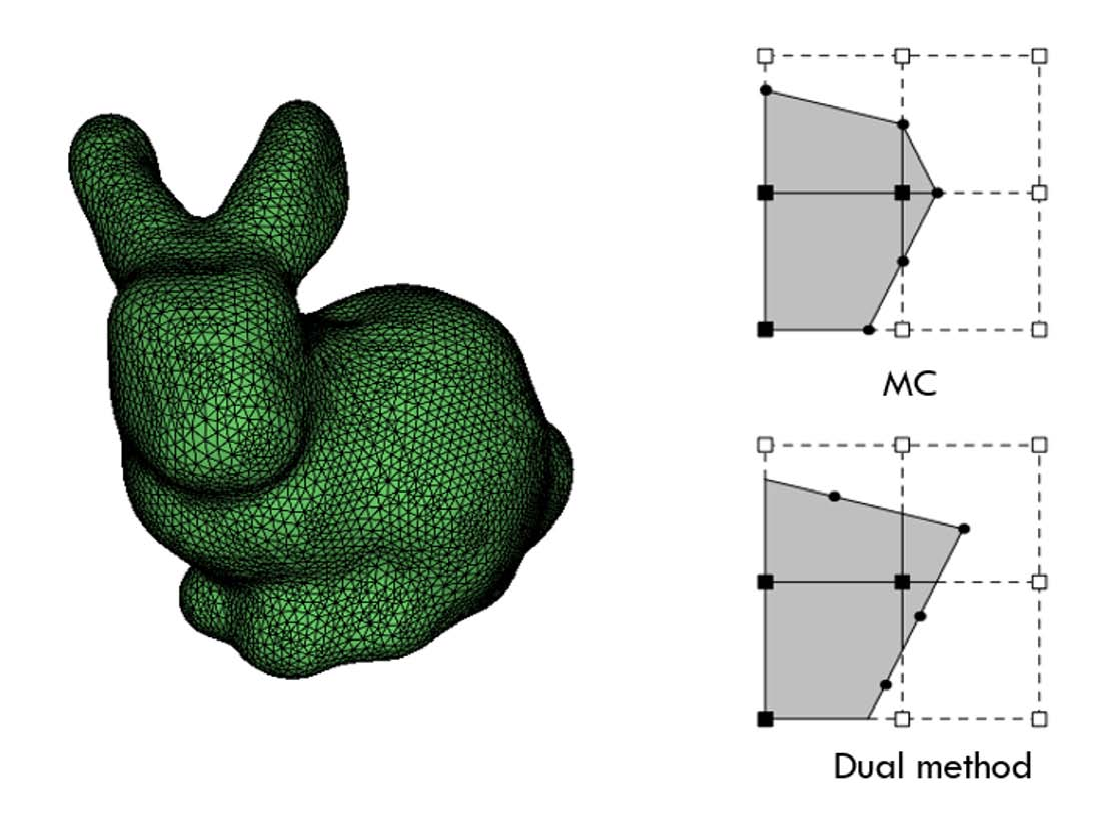
\includegraphics[scale=0.4]{Pictures/bunny_MC.pdf}

		\end{figure}

	\end{minipage}
	\begin{minipage}{0.14\textwidth}
		\begin{figure}
					\scalebox{0.08}{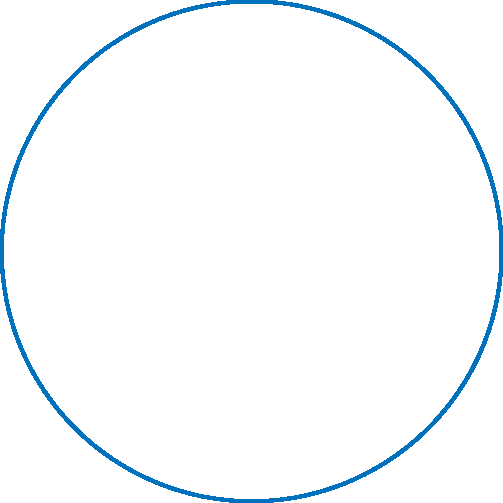
\includegraphics{Pictures/1CAD.pdf}}\\
					\scalebox{0.08}{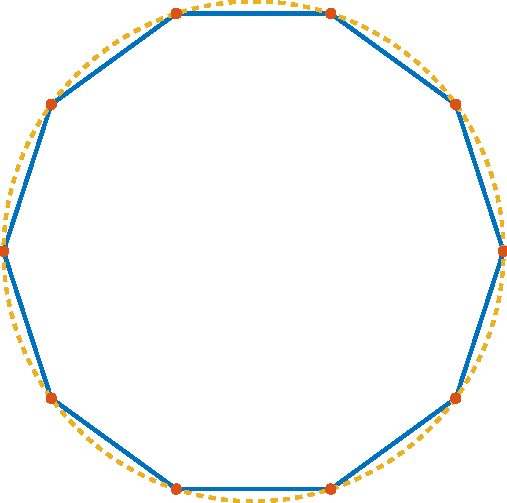
\includegraphics{Pictures/2STL.pdf}}\\
					\scalebox{0.08}{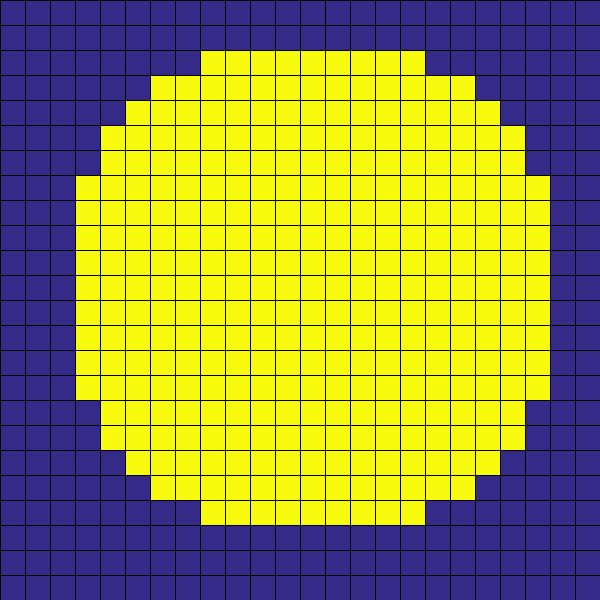
\includegraphics{Pictures/3VOX.pdf}}\\
					\scalebox{0.08}{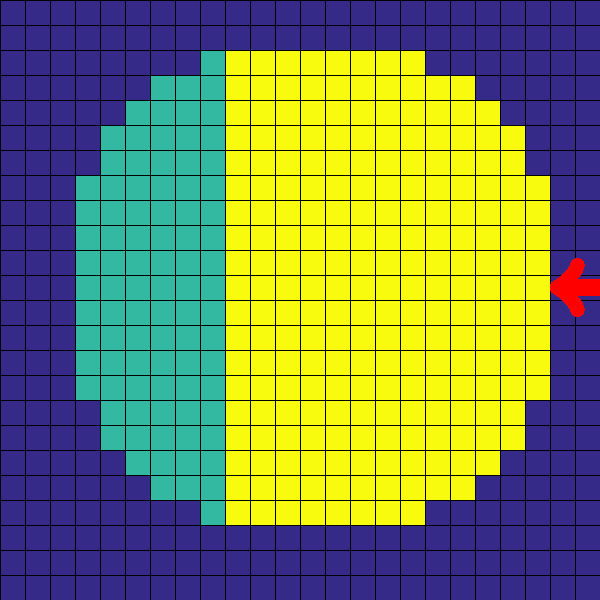
\includegraphics{Pictures/4TPD.pdf}}\\
					\scalebox{0.08}{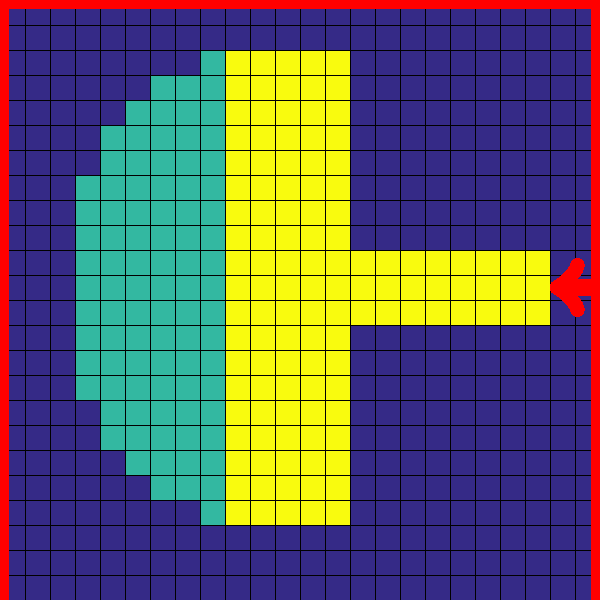
\includegraphics{Pictures/5TOPOPTmark2.pdf}}\\
					%\scalebox{0.08}{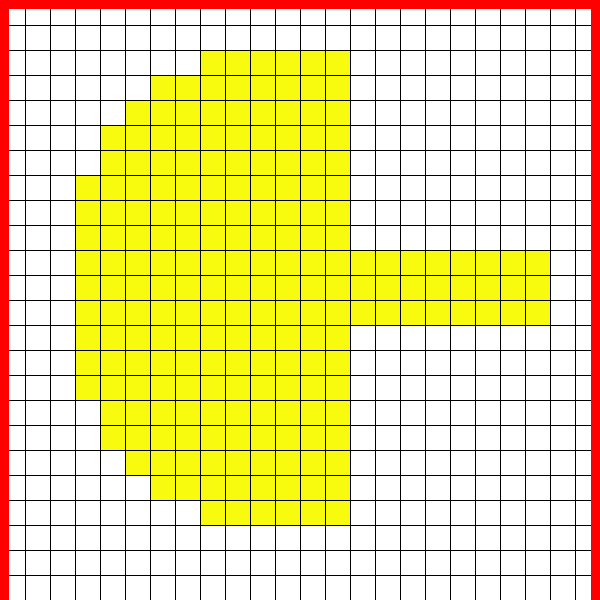
\includegraphics{Pictures/6TOPYOUTmark2.pdf}}\\
					\scalebox{0.08}{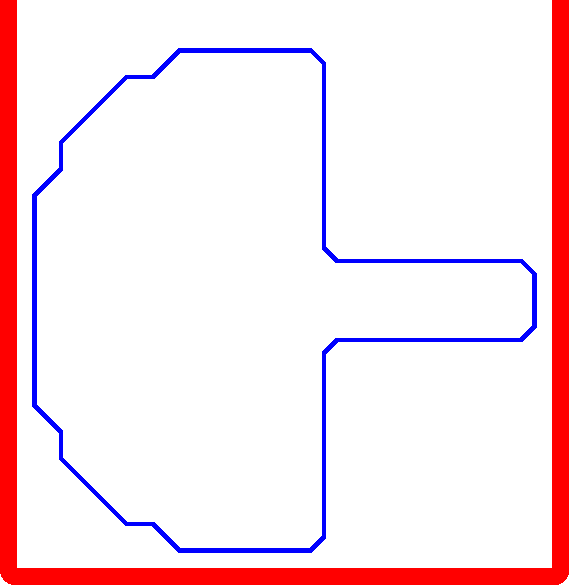
\includegraphics{Pictures/7MCmark1.pdf}}  %THIS NEEDS TO BE CHANGED FOR MARK!
					\scalebox{0.08}{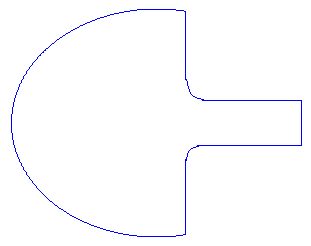
\includegraphics[scale=1.3]{Pictures/End.png}}
		\end{figure}
	\end{minipage}



\end{frame}

\begin{frame}

	\frametitle{Surface Extraction}
	\begin{minipage}{0.85\textwidth}
	\text Contour Filtering using Implicit Modelling 


	\begin{figure}
	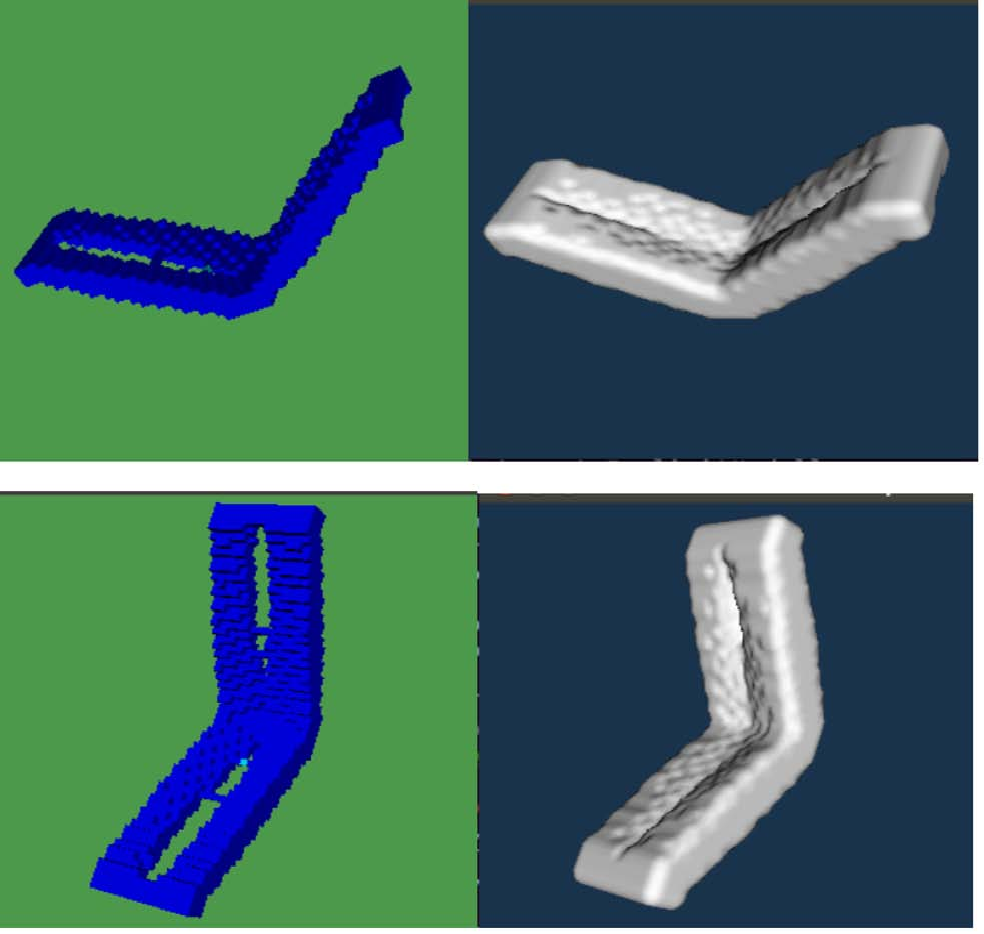
\includegraphics[scale=0.35]{Pictures/contouring.pdf}

	\end{figure}


	\textbf {Problem: Holes are not taken into account}

	\end{minipage}
	\begin{minipage}{0.14\textwidth}
		\begin{figure}
					\scalebox{0.08}{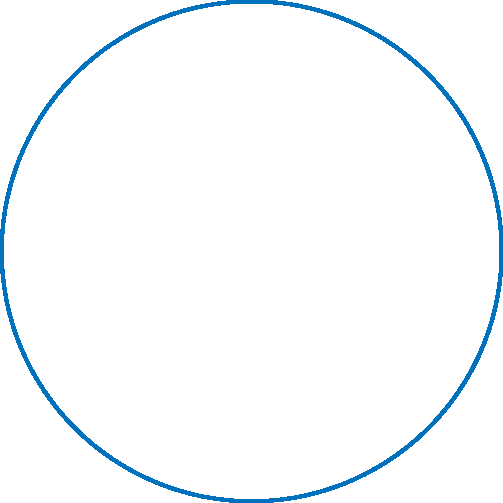
\includegraphics{Pictures/1CAD.pdf}}\\
					\scalebox{0.08}{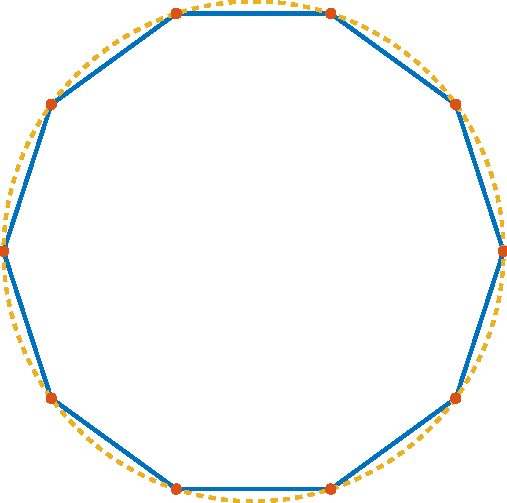
\includegraphics{Pictures/2STL.pdf}}\\
					\scalebox{0.08}{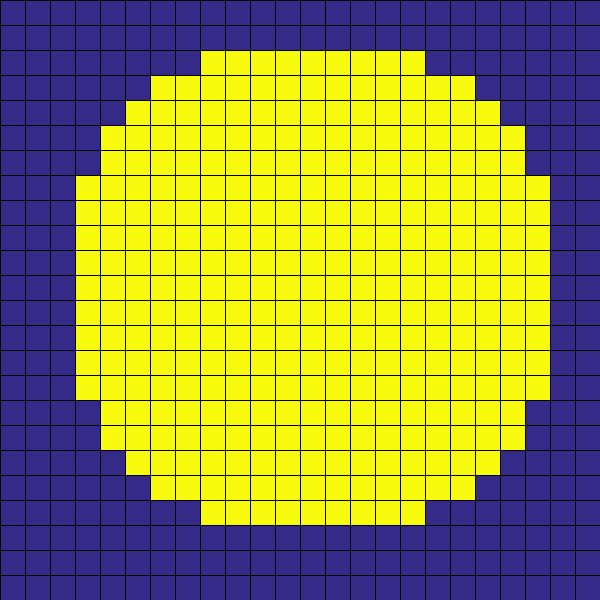
\includegraphics{Pictures/3VOX.pdf}}\\
					\scalebox{0.08}{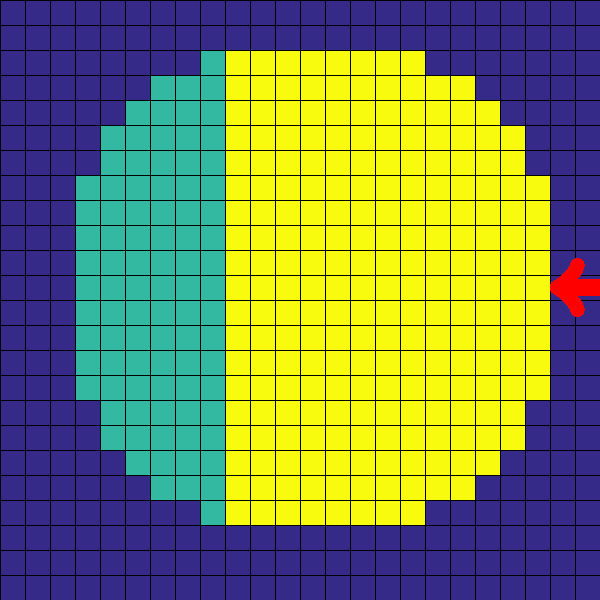
\includegraphics{Pictures/4TPD.pdf}}\\
					\scalebox{0.08}{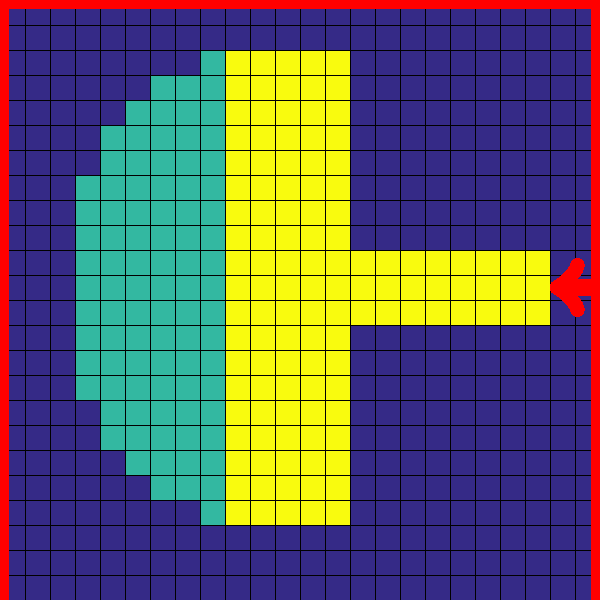
\includegraphics{Pictures/5TOPOPTmark2.pdf}}\\
					%\scalebox{0.08}{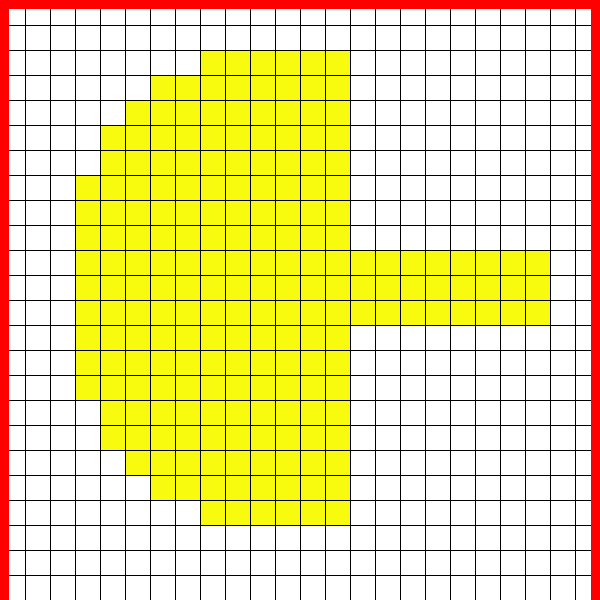
\includegraphics{Pictures/6TOPYOUTmark2.pdf}}\\
					\scalebox{0.08}{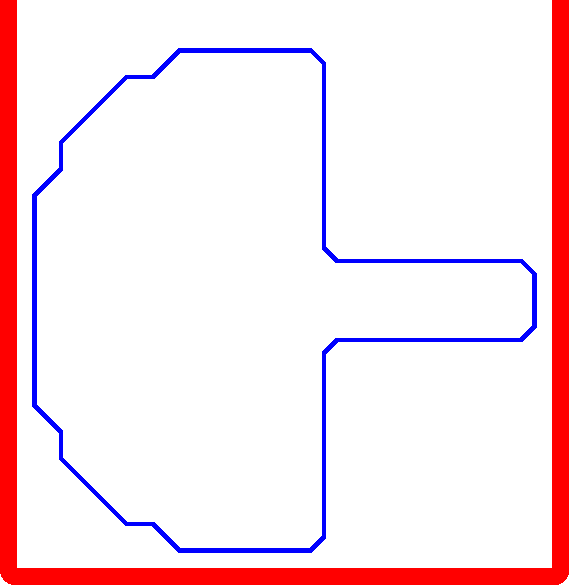
\includegraphics{Pictures/7MCmark1.pdf}}  %THIS NEEDS TO BE CHANGED FOR MARK!
					\scalebox{0.08}{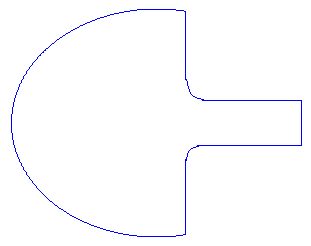
\includegraphics[scale=1.3]{Pictures/End.png}}
		\end{figure}
	\end{minipage}





\end{frame}

\begin{frame}

	\frametitle{Decimation}
	\begin{minipage}{0.85\textwidth}
	\begin{itemize}
	\item Fine mesh to a coarser mesh through Decimation- Reduction of number of triangles. (Upper: 50\% Lower: 90\% )
	\end{itemize}

	\begin{itemize}
	\item Smoothing step is needed in between
	\end{itemize}

	\begin{figure}
	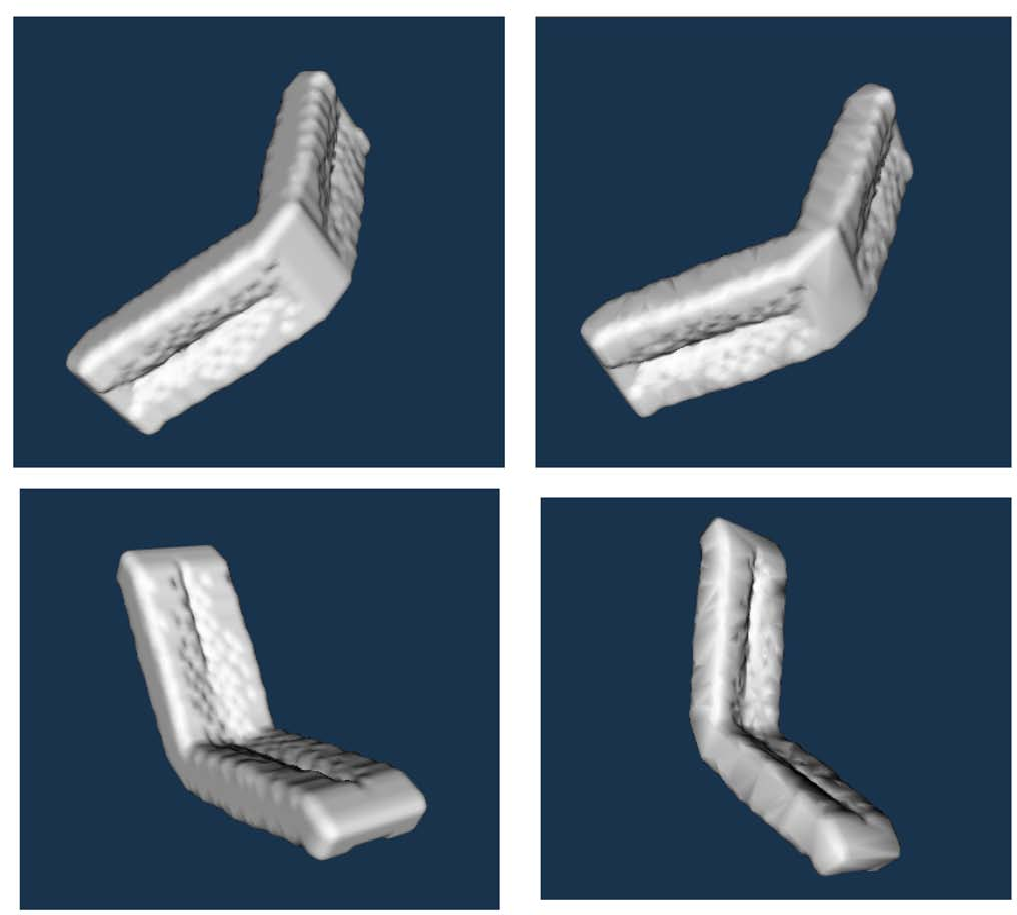
\includegraphics[scale=0.34]{Pictures/Decimation.pdf}

	\end{figure}
	\end{minipage}
	\begin{minipage}{0.14\textwidth}
		\begin{figure}
					\scalebox{0.08}{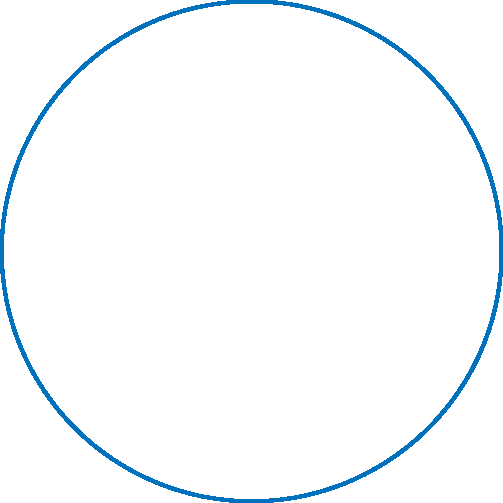
\includegraphics{Pictures/1CAD.pdf}}\\
					\scalebox{0.08}{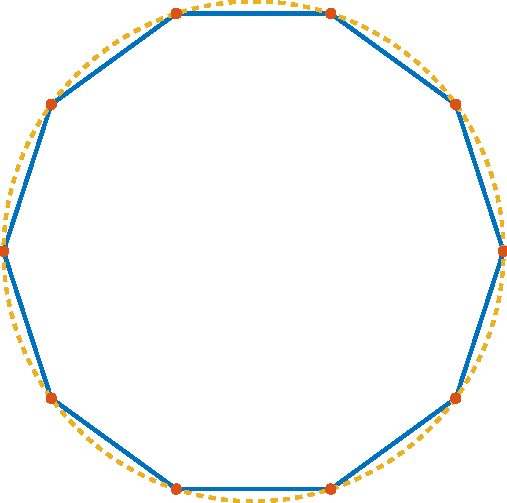
\includegraphics{Pictures/2STL.pdf}}\\
					\scalebox{0.08}{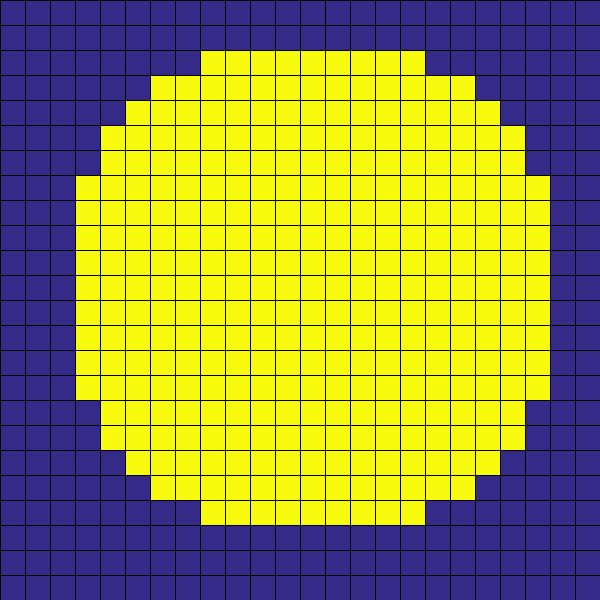
\includegraphics{Pictures/3VOX.pdf}}\\
					\scalebox{0.08}{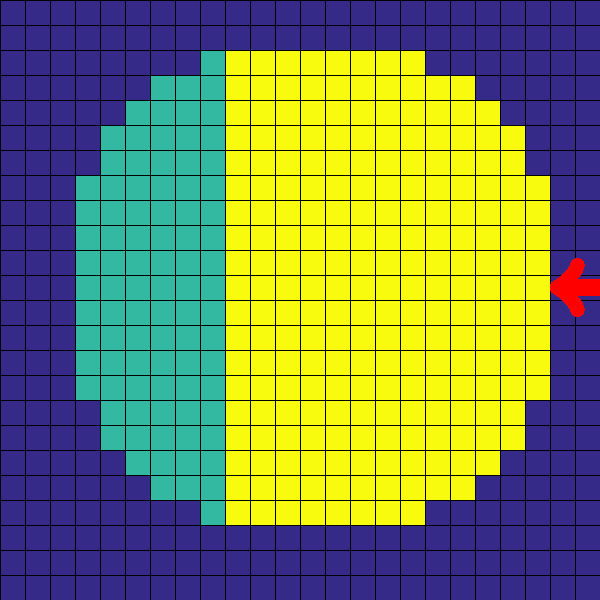
\includegraphics{Pictures/4TPD.pdf}}\\
					\scalebox{0.08}{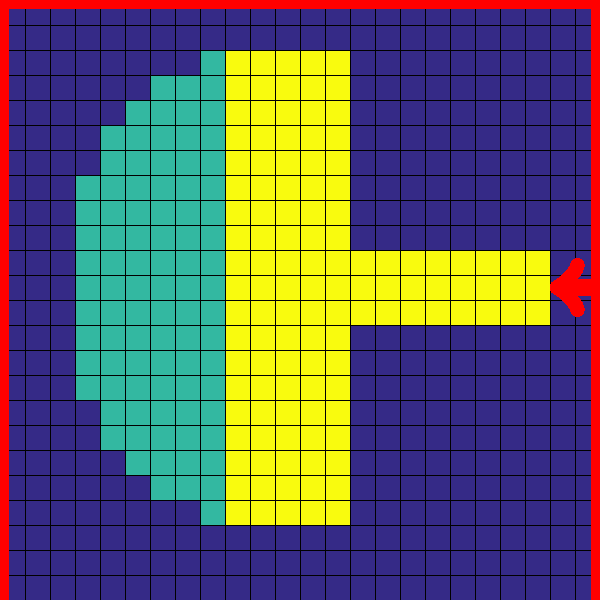
\includegraphics{Pictures/5TOPOPTmark2.pdf}}\\
					%\scalebox{0.08}{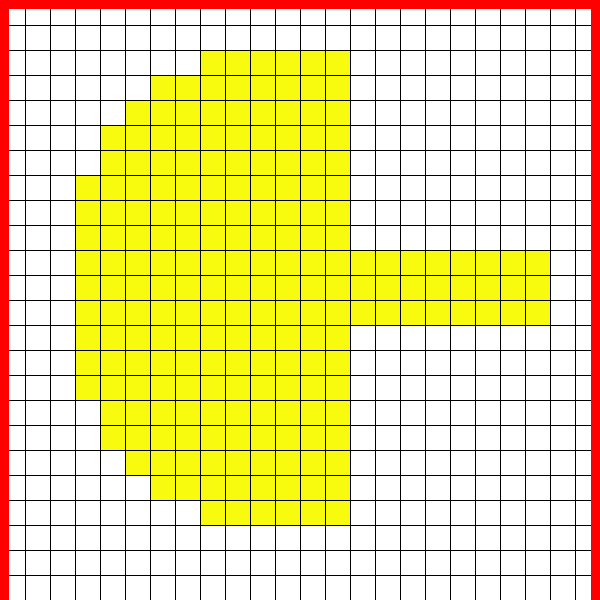
\includegraphics{Pictures/6TOPYOUTmark2.pdf}}\\
					\scalebox{0.08}{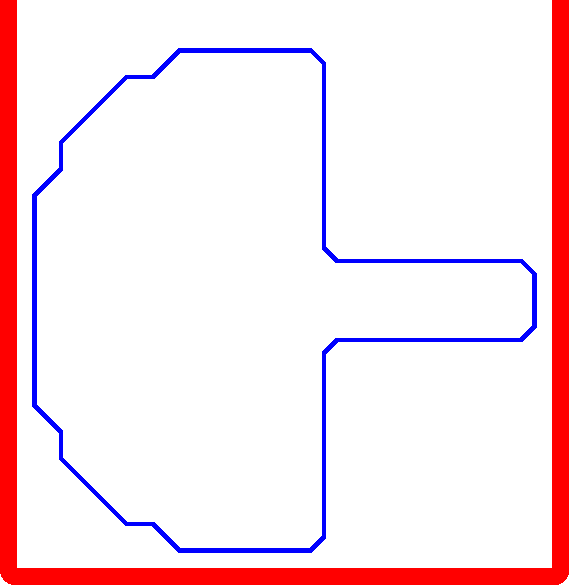
\includegraphics{Pictures/7MCmark1.pdf}}  %THIS NEEDS TO BE CHANGED FOR MARK!
					\scalebox{0.08}{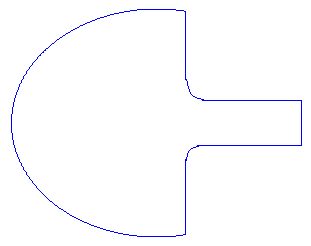
\includegraphics[scale=1.3]{Pictures/End.png}}
		\end{figure}
	\end{minipage}





\end{frame}
